% ======================================================================
%  Appendix D — Material Tensors and Sign Conventions
% ======================================================================

\section{Why conventions matter}
\label{sec:appD-why}

Topological photonics is unusually sensitive to signs.  A reversed time
harmonic convention changes the sign of the imaginary part of a lossy
permittivity; a reversed magnetic bias changes the sign of the
gyrotropic tensor element; a reversed convention for the Berry
connection changes the sign of every Chern number.  None of these
changes is physically mysterious, but a book-length derivation must keep
them consistent.

This appendix collects the material tensors, sign conventions, and
frequency-domain response models used throughout the monograph.  It is
not a substitute for the derivations in Chapters~\ref{ch:maxwell-dynamics}
through~\ref{ch:geometry-bands}; it is a reference table for checking
formulae and translating between sources.

\section{Time-harmonic convention}
\label{sec:appD-convention}

Throughout this book we use the engineering convention
\begin{equation}\label{eq:appD-time-convention}
  \Efield(\rvec,t)=\real\{\Efield(\rvec)\ee^{-\ii\omega t}\}\,,
  \qquad \omega>0\,.
\end{equation}
With this convention the source-free frequency-domain Maxwell curl
equations are
\begin{equation}\label{eq:appD-maxwell-frequency}
  \nabla\times\Efield = \ii\omega\Bfield\,,
  \qquad
  \nabla\times\Hfield = -\ii\omega\Dfield\,.
\end{equation}
The six-component first-order equation is therefore
\begin{equation}\label{eq:appD-first-order}
  \Maxop\emfield=\omega\Mmat\emfield\,,
  \qquad
  \Maxop=\begin{pmatrix}0&\ii\nabla\times\\-\ii\nabla\times&0\end{pmatrix}\,.
\end{equation}

\begin{center}
\begin{tabular}{lcc}
  \toprule
  & \textbf{Convention used here} & \textbf{Opposite convention} \\
  & $\ee^{-\ii\omega t}$ & $\ee^{+\ii\omega t}$ \\
  \midrule
  Faraday law & $\nabla\times\Efield=\ii\omega\Bfield$ &
    $\nabla\times\Efield=-\ii\omega\Bfield$ \\
  Amp\`ere law & $\nabla\times\Hfield=-\ii\omega\Dfield$ &
    $\nabla\times\Hfield=\ii\omega\Dfield$ \\
    Absorbing dielectric & $\imag\varepsilon>0$ & $\imag\varepsilon<0$ \\
  Growing mode & $\imag\omega>0$ & $\imag\omega<0$ \\
  Decaying mode & $\imag\omega<0$ & $\imag\omega>0$ \\
  \bottomrule
\end{tabular}
\end{center}

Many papers in topological photonics and microwave engineering use the
opposite convention.  When importing a formula, especially for
magneto-optical tensors, first translate the time convention
\cite{wang2007reflection}.

\section{The six-component material matrix}
\label{sec:appD-material-matrix}

For a local linear medium the constitutive relation is
\begin{equation}\label{eq:appD-constitutive}
  \begin{pmatrix}\Dfield\\\Bfield\end{pmatrix}
  =\Mmat(\rvec,\omega)
  \begin{pmatrix}\Efield\\\Hfield\end{pmatrix},
  \qquad
  \Mmat=\begin{pmatrix}
    \varepsilon_0\epst & \clight^{-1}\xit\\
    \clight^{-1}\zetat & \mu_0\mut
  \end{pmatrix}\,.
\end{equation}
Here $\epst$ and $\mut$ are dimensionless relative permittivity and
permeability tensors; $\xit$ and $\zetat$ are dimensionless
magneto-electric tensors.  With the normalisation used here, the
cross-coupling blocks have the same units as the diagonal blocks after
the factors $\varepsilon_0$, $\mu_0$, and $c^{-1}$ are included.

\subsection{Losslessness, reciprocity, and time reversal}
\label{sec:appD-symmetry-conditions}

The central tensor conditions are:
\begin{center}
\begin{tabular}{lccc}
  \toprule
  \textbf{Property} & $\epst$ & $\mut$ & $\xit,\zetat$ \\
  \midrule
  Lossless & $\epst=\epst^\dagger$ & $\mut=\mut^\dagger$ &
    $\zetat=\xit^\dagger$ \\
  Reciprocal & $\epst=\epst^T$ & $\mut=\mut^T$ &
    $\xit=-\zetat^T$ \\
  Time-reversal invariant & $\epst=\epst^*$ & $\mut=\mut^*$ &
    $\xit=-\xit^*$ and $\zetat=-\zetat^*$ \\
  Positive energy, nondispersive & $\Mmat>0$ & & \\
  Positive energy, dispersive & $\Mgmat=\partial_\omega(\omega\Mmat)>0$ & & \\
  \bottomrule
\end{tabular}
\end{center}
For lossless media, reciprocity and time-reversal invariance are
equivalent, as shown in Proposition~\ref{prop:ch2-TR-reciprocal}.

\section{Permittivity tensors}
\label{sec:appD-eps}

\subsection{Isotropic and uniaxial media}
\label{sec:appD-isotropic-uniaxial}

An isotropic dielectric has
\begin{equation}\label{eq:appD-isotropic-eps}
  \epst=\varepsilon_r\mathbf{I}_3\,.
\end{equation}
A uniaxial crystal with optic axis along $z$ has
\begin{equation}\label{eq:appD-uniaxial-eps}
  \epst=\diag(\varepsilon_\perp,\varepsilon_\perp,\varepsilon_z)\,.
\end{equation}
For a lossless reciprocal crystal the entries are real.  For a lossy
medium under our time convention ($\ee^{-\ii\omega t}$), the imaginary
parts are positive: $\operatorname{Im}\varepsilon>0$,
$\operatorname{Im}\mu>0$.

\subsection{Gyroelectric media}
\label{sec:appD-gyroelectric}

For a magneto-optical material biased along $+\hat{z}$, a common
permittivity tensor is
\begin{equation}\label{eq:appD-eps-gyro}
  \epst=\begin{pmatrix}
    \varepsilon_\perp & -\ii\varepsilon_g & 0\\
    \ii\varepsilon_g & \varepsilon_\perp & 0\\
    0&0&\varepsilon_z
  \end{pmatrix}\,.
\end{equation}
For real $\varepsilon_\perp$, $\varepsilon_g$, and $\varepsilon_z$, this
matrix is Hermitian but not symmetric, so it is lossless and
nonreciprocal.  Reversing the bias changes
$\varepsilon_g\mapsto-\varepsilon_g$.

The circularly polarised eigenvectors in the $x$-$y$ plane are
$\mathbf{e}_\pm=(\hat{x}\pm\ii\hat{y})/\sqrt{2}$ with effective
permittivities
\begin{equation}\label{eq:appD-circular-eps}
  \varepsilon_\pm=\varepsilon_\perp\pm\varepsilon_g\,.
\end{equation}
The difference in phase velocity between the two circular polarisations
is the Faraday effect.

\section{Permeability tensors}
\label{sec:appD-mu}

\subsection{Gyromagnetic ferrites}
\label{sec:appD-ferrites}

At microwave frequencies, magnetised ferrites are described by the
Polder tensor
\begin{equation}\label{eq:appD-mu-polder}
  \mut=\begin{pmatrix}
    \mu_\perp & -\ii\kappa_\mu & 0\\
    \ii\kappa_\mu & \mu_\perp & 0\\
    0&0&\mu_z
  \end{pmatrix}\,
\end{equation}
The displayed formula above follows the convention and normalisation used in \cite{he2016photonic}.
For the simplest saturated ferrite with bias along $+\hat{z}$ and
negligible damping,
\begin{equation}\label{eq:appD-polder-params}
  \mu_\perp(\omega)=1+\frac{\omega_0\omega_m}{\omega_0^2-\omega^2}\,,
  \qquad
  \kappa_\mu(\omega)=\frac{\omega\omega_m}{\omega_0^2-\omega^2}\,,
  \qquad \mu_z=1\,.
\end{equation}
Here $\omega_0=\gamma B_0$ is the Larmor frequency and
$\omega_m=\gamma\mu_0M_s$ is set by the saturation magnetisation.  A
small damping rate is included by replacing
$\omega_0\mapsto\omega_0-\ii\alpha\omega$ in the denominator, with the
sign adjusted for the time convention.

\subsection{Circular basis}
\label{sec:appD-mu-circular}

In the circular basis $\mathbf{h}_\pm=(\hat{x}\pm\ii\hat{y})/\sqrt{2}$,
the Polder eigenvalue for $\mathbf{h}_+$ is $\mu_\perp+\kappa_\mu$
(left-circular under the $\ee^{-\ii\omega t}$ convention)
and for $\mathbf{h}_-$ is $\mu_\perp-\kappa_\mu$ (right-circular).
Following the standard ferrite convention adopted in
Chapters~3 and~9, we label the right-circular eigenvalue as
$\mu_+$ and the left-circular as $\mu_-$:
\begin{equation}\label{eq:appD-mu-circular}
  \mu_\pm=\mu_\perp\mp\kappa_\mu\,.
\end{equation}
Positive magnetic energy in the nondispersive approximation requires
$\mu_\perp>|\kappa_\mu|$ and $\mu_z>0$.  In a dispersive ferrite the
correct requirement is positivity of the magnetic block of $\Mgmat$.

\subsection{Typical YIG numbers}
\label{sec:appD-yig}

For yttrium iron garnet (YIG), representative microwave parameters are
\begin{equation}\label{eq:appD-yig-values}
  \gamma\approx 2\pi\times 28\;\mathrm{GHz/T}\,,
  \qquad
  \mu_0M_s\approx 0.175\;\mathrm{T}\,,
\end{equation}
so $\omega_m/(2\pi)\approx 4.9\;\mathrm{GHz}$.  A bias field
$B_0=0.20\;\mathrm{T}$ gives $\omega_0/(2\pi)\approx5.6\;\mathrm{GHz}$.
At operating frequencies below resonance (for example
$4.5\;\mathrm{GHz}$), the gyrotropic parameter can be order unity,
which is why YIG is so effective for microwave topological photonic
crystals.

Figure~\ref{fig:appD-polder-sign-conventions} collects the sign
choices used in this appendix and in Chapters~7--10.  The time
convention is $\ee^{-\ii\omega t}$, so passive absorption has positive
imaginary permittivity.  For a ferrite biased along $+\hat{z}$ the
Polder tensor has off-diagonal entries $-\ii\kappa_\mu$ and
$+\ii\kappa_\mu$ in the $xy$ block.  Reversing the bias reverses
$\kappa_\mu$, and the circular eigenvalues exchange their roles.

\begin{figure}[t]
  \centering
  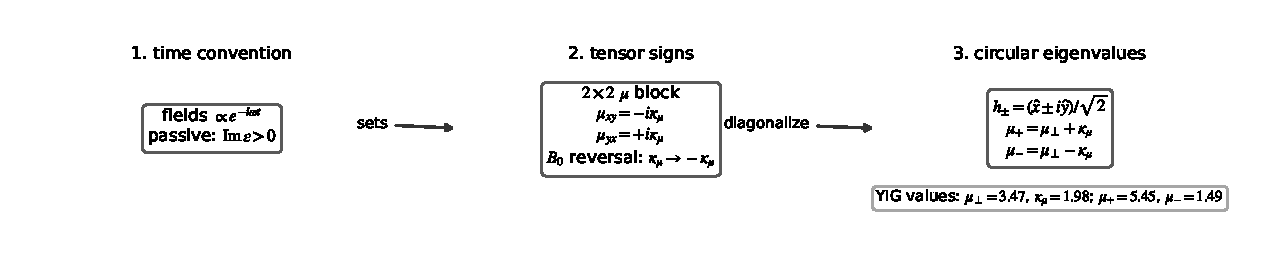
\includegraphics[width=0.96\textwidth]{figures/fig_appD_polder_sign_conventions.pdf}
  \caption{Material-tensor signs under the convention used throughout
  this monograph.  With fields proportional to $\ee^{-\ii\omega t}$,
  passive loss has $\operatorname{Im}\varepsilon>0$.  For a ferrite
  biased along $+\hat z$, the Polder tensor has the gyrotropic entries
  shown in the middle panel; reversing the bias flips $\kappa_\mu$.
    In the circular basis the eigenvalues are
    $\mu_+=\mu_\perp-\kappa_\mu$ (right-circular) and
    $\mu_-=\mu_\perp+\kappa_\mu$ (left-circular).  For the verified
    YIG parameters, $\mu_+=1.49$ and $\mu_-=5.45$.}
  \label{fig:appD-polder-sign-conventions}
\end{figure}


\section{Bianisotropic tensors}
\label{sec:appD-bianisotropic}

Bianisotropic media couple electric and magnetic fields \cite{slobozhanyuk2015observation}:
\begin{equation}\label{eq:appD-bianisotropic-expanded}
  \Dfield=\varepsilon_0\epst\Efield+\clight^{-1}\xit\Hfield\,,
  \qquad
  \Bfield=\clight^{-1}\zetat\Efield+\mu_0\mut\Hfield\,.
\end{equation}
Important special cases include:
\begin{enumerate}[label=(\roman*)]
  \item \textbf{Chiral media:} $\xit=\ii\chi\mathbf{I}$,
    $\zetat=-\ii\chi\mathbf{I}$ for reciprocal optical activity.
  \item \textbf{Tellegen media:} $\xit=\zetat=\chi_T\mathbf{I}$,
    which break time reversal and reciprocity.
  \item \textbf{Omega media:} antisymmetric magneto-electric coupling
    used in metamaterial realisations of pseudospin photonics.
\end{enumerate}
Bianisotropy is central to reciprocal photonic topological insulators,
where it couples TE and TM sectors in a controlled way \cite{khanikaev2013photonic}.

\section{Dispersive energy metric}
\label{sec:appD-energy-metric}

For a lossless but dispersive material, the correct energy inner product
uses the Brillouin energy density rather than the instantaneous field
energy \cite{gangaraj2016berry,silveirinha2016bulk}.  The dispersive
energy metric is
\begin{equation}\label{eq:appD-Mg}
  \Mgmat(\omega)=\pderiv{}{\omega}\bigl[\omega\Mmat(\omega)\bigr]
  =\Mmat(\omega)+\omega\pderiv{\Mmat}{\omega}\,.
\end{equation}
This formula applies block by block: the electric block is
$\varepsilon_0\,\partial_\omega(\omega\epst)$, the magnetic block is
$\mu_0\,\partial_\omega(\omega\mut)$, and the cross-coupling blocks
follow similarly.

\subsection{Physical origin}
\label{sec:appD-Mg-physical}

The extra term $\omega\,\partial_\omega\Mmat$ accounts for the energy
stored in the internal degrees of freedom of the medium---bound
electrons for a dielectric, precessing spins for a ferrite.  When the
field oscillates at frequency $\omega$, these internal oscillators
respond with an amplitude that depends on $\omega$; the total
time-averaged energy density is the sum of the vacuum-field energy and
the oscillator energy.  Brillouin showed that for a lossless dispersive
medium the result is exactly $\frac{1}{4}\emfield^\dagger\Mgmat\,\emfield$
\cite{gangaraj2016berry}.

\subsection{Positivity from passivity}
\label{sec:appD-Mg-positivity}

For the electromagnetic inner product and Berry connection to be
well-defined, the energy metric $\Mgmat$ must be positive definite.
This is guaranteed by passivity: a lossless medium that does not
spontaneously emit energy must store a non-negative energy density
for every nonzero field configuration.

More precisely, consider a quasi-monochromatic wave packet centred at
frequency $\omega$ with slowly varying envelope $\mathbf{a}(t)$.  The
time-averaged energy density is
\begin{equation}\label{eq:appD-energy-density}
  \langle u\rangle
  = \frac{1}{4}\,\mathbf{a}^\dagger\,
  \pderiv{}{\omega}\bigl[\omega\Mmat(\omega)\bigr]\,\mathbf{a}
  = \frac{1}{4}\,\mathbf{a}^\dagger\,\Mgmat(\omega)\,\mathbf{a}\,.
\end{equation}
Passivity requires $\langle u\rangle\geq 0$ for all $\mathbf{a}\neq 0$,
hence $\Mgmat(\omega)\geq 0$.  Strict positivity ($\Mgmat>0$) holds
at frequencies away from material resonances, where $\Mmat(\omega)$ is
smooth and the medium is transparent.

\section{Polder tensor: detailed derivation}
\label{sec:appD-polder-detailed}

For the Polder ferrite, the dispersive derivatives are
\cite{gangaraj2016berry} strict positivity of $\Mgmat$ can be verified
explicitly.  The circular-basis eigenvalues of the magnetic block are
$\mu_{g,\pm}=\partial_\omega(\omega\mu_\pm)$, with $\mu_\pm=\mu_\perp\mp\kappa_\mu$.
Since $\mu_+=1+\omega_m/(\omega_0+\omega)$ and
$\mu_-=1+\omega_m/(\omega_0-\omega)$, differentiation gives
\begin{equation}\label{eq:appD-Mg-ferrite-eigenvalues}
  \mu_{g,\pm}
  = 1 + \frac{\omega_m\,\omega_0}{(\omega_0\pm\omega)^2}\,.
\end{equation}
Both eigenvalues are manifestly positive for $\omega<\omega_0$ (below
ferromagnetic resonance), confirming that the energy metric is positive
definite in the operating range of gyromagnetic photonic crystals.

\subsection{Role in the Berry connection}
\label{sec:appD-Mg-berry}

The Berry connection of a photonic band is defined using the
$\Mgmat$-weighted inner product \cite{gangaraj2016berry}:
\begin{equation}\label{eq:appD-berry-Mg}
  \Aberry_{n,\alpha}
  = \ii\int_\Omega
  \mathbf{u}_{n\kvec}^\dagger\,\Mgmat(\omega_n)\,
  \nabla_{k_\alpha}\mathbf{u}_{n\kvec}\,\dd^d r\,.
\end{equation}
If one uses the bare material matrix $\Mmat$ instead of $\Mgmat$, the
resulting Berry connection is not gauge-invariant under frequency
relabelling, and the Chern number may depend on the choice of
normalisation.  The dispersive correction $\omega\,\partial_\omega\Mmat$
is therefore not a refinement but a necessity for any material with
frequency-dependent constitutive parameters \cite{silveirinha2016bulk}.
\begin{align}\label{eq:appD-polder-derivatives}
  \pderiv{\mu_\perp}{\omega}
  &=\frac{2\omega\omega_0\omega_m}{(\omega_0^2-\omega^2)^2}\,,\\
  \pderiv{\kappa_\mu}{\omega}
  &=\frac{\omega_m(\omega_0^2+\omega^2)}{(\omega_0^2-\omega^2)^2}\,.
\end{align}
Thus the transverse magnetic energy block is
\begin{equation}\label{eq:appD-Mg-polder}
  \mut_g=\begin{pmatrix}
    \mu_\perp+\omega\partial_\omega\mu_\perp &
      -\ii(\kappa_\mu+\omega\partial_\omega\kappa_\mu)&0\\
    \ii(\kappa_\mu+\omega\partial_\omega\kappa_\mu)&
      \mu_\perp+\omega\partial_\omega\mu_\perp&0\\
    0&0&1
  \end{pmatrix}\,.
\end{equation}
The eigenvalues in the circular basis are
\begin{equation}\label{eq:appD-Mg-circular}
  \mu_{g,\pm}=\mu_\perp+\omega\partial_\omega\mu_\perp
  \pm\bigl(\kappa_\mu+\omega\partial_\omega\kappa_\mu\bigr)\,.
\end{equation}
A passive stable ferrite away from resonance must have
$\mu_{g,+}>0$ and $\mu_{g,-}>0$.

\section{Drude and Lorentz response}
\label{sec:appD-drude-lorentz}

\subsection{Drude model}
\label{sec:appD-drude}

For free carriers,
\begin{equation}\label{eq:appD-drude}
  \varepsilon(\omega)=\varepsilon_\infty-
  \frac{\omega_p^2}{\omega(\omega+\ii\gamma_D)}\,
\end{equation}
The displayed formula above follows the convention and normalisation used in \cite{press2026photonic}.
With our $\ee^{-\ii\omega t}$ convention, $\gamma_D>0$ gives
absorption.  In the lossless limit $\gamma_D=0$,
\begin{equation}\label{eq:appD-drude-energy}
  \pderiv{}{\omega}\bigl[\omega\varepsilon(\omega)\bigr]
  =\varepsilon_\infty+\frac{\omega_p^2}{\omega^2}>0\,.
\end{equation}

\subsection{Lorentz oscillator}
\label{sec:appD-lorentz}

For a bound resonance,
\begin{equation}\label{eq:appD-lorentz}
  \varepsilon(\omega)=\varepsilon_\infty+
  \frac{f\omega_r^2}{\omega_r^2-\omega^2-\ii\gamma_L\omega}\,.
\end{equation}
In the lossless limit,
\begin{equation}\label{eq:appD-lorentz-energy}
  \partial_\omega[\omega\varepsilon(\omega)]
  =\varepsilon_\infty+f\omega_r^2\frac{\omega_r^2+\omega^2}{(\omega_r^2-\omega^2)^2}>0
\end{equation}
away from the material resonance.  This positivity is the oscillator
origin of the Brillouin energy formula.

\section{Useful constants and units}
\label{sec:appD-units}

\begin{center}
\begin{tabular}{lll}
  \toprule
  \textbf{Quantity} & \textbf{Symbol} & \textbf{SI value} \\
  \midrule
  Speed of light & $c$ & $2.99792458\times10^8\;\mathrm{m/s}$ \\
  Vacuum permittivity & $\varepsilon_0$ & $8.8541878128\times10^{-12}\;\mathrm{F/m}$ \\
  Vacuum permeability & $\mu_0$ & $1.25663706212\times10^{-6}\;\mathrm{H/m}$ \\
  Free-space impedance & $Z_0=\sqrt{\mu_0/\varepsilon_0}$ & $376.730313668\;\Omega$ \\
  Reduced Planck constant & $\hbar$ & $1.054571817\times10^{-34}\;\mathrm{J\,s}$ \\
  Electron charge & $e$ & $1.602176634\times10^{-19}\;\mathrm{C}$ \\
  Electron gyromagnetic ratio & $\gamma/(2\pi)$ & $28.025\;\mathrm{GHz/T}$ \\
  \bottomrule
\end{tabular}
\end{center}

\section{Checklist for translating sources}
\label{sec:appD-checklist}

Sources in topological photonics use a wide variety of sign conventions
\cite{ozawa2018topological,gangaraj2016berry}.  When using a formula
from another paper, check the following before
inserting it into this monograph:
\begin{enumerate}
  \item Does the paper use $\ee^{-\ii\omega t}$ or $\ee^{+\ii\omega t}$?
  \item Is the gyrotropic tensor written with $+\ii g$ or $-\ii g$ in
  the $xy$ component?
  \item Is the Berry connection defined as $+\ii\langle u|\nabla u\rangle$
  or $-\ii\langle u|\nabla u\rangle$?
  \item Is the inner product the bare $L^2$ product or the electromagnetic
  energy product with $\Mmat$ or $\Mgmat$?
  \item Is material dispersion ignored, approximated, or included through
  auxiliary oscillator variables?
  \item Are the quoted Chern numbers for individual bands, composite
  band groups, or gaps?
\end{enumerate}
Only after these convention checks should formulas be compared or cited.

\section{Kramers--Kronig relations and passivity} \cite{raman2010photonic,nittis2020equivalence}
\label{sec:appD-kramers-kronig}

\subsection{The dispersion relations}
\label{sec:appD-kk-derivation}

Any causal linear response function $\chi(\omega)$ satisfies the
Kramers--Kronig relations, which connect the real and imaginary parts:
\begin{align}
  \real\,\chi(\omega)
  &= \frac{1}{\pi}\,\mathrm{P.V.}\!\int_{-\infty}^{\infty}
  \frac{\imag\,\chi(\omega')}{\omega'-\omega}\,\dd\omega'\,,
  \label{eq:appD-kk-real}\\
  \imag\,\chi(\omega)
  &= -\frac{1}{\pi}\,\mathrm{P.V.}\!\int_{-\infty}^{\infty}
  \frac{\real\,\chi(\omega')}{\omega'-\omega}\,\dd\omega'\,.
  \label{eq:appD-kk-imag}
\end{align}
Here P.V.\ denotes the Cauchy principal value.  For the dielectric
permittivity $\varepsilon(\omega)=1+\chi_e(\omega)$, the Kramers--Kronig
relations guarantee that $\imag\,\varepsilon(\omega)>0$ for $\omega>0$
in a passive medium, and that the dispersive energy metric
$\Mgmat(\omega)=\partial_\omega[\omega\Mmat(\omega)]$ is positive
definite at all real frequencies outside the absorption bands
\cite{gangaraj2016berry,silveirinha2016bulk}.

\subsection{Passivity and the positive-definite metric}
\label{sec:appD-passivity}

A medium is passive if it does not provide energy to the field.
Mathematically, this requires that the power dissipated by any field
configuration is non-negative:
$\emfield^\dagger\,\imag[\omega\Mmat(\omega)]\,\emfield\geq 0$ for
all $\omega>0$ and all $\emfield$.  Combined with the Kramers--Kronig
relations, passivity implies \cite{gangaraj2016berry}
\begin{equation}\label{eq:appD-passivity}
  \Mgmat(\omega) = \frac{\partial[\omega\Mmat(\omega)]}{\partial\omega}
  \succ 0
  \quad\text{(positive definite)}
\end{equation}
at all real frequencies in the transparency windows (where
$\imag\,\Mmat\approx 0$).  This result, proved rigorously by
Silveirinha \cite{silveirinha2016bulk}, is the foundation for the
Hermitian structure of the photonic eigenproblem and the well-definedness
of the Chern number.

\section{Worked examples of sign-convention translation}
\label{sec:appD-worked-examples}

\subsection{Example 1: Haldane--Raghu to this book}
\label{sec:appD-example-haldane}

Haldane and Raghu \cite{haldane2008possible} use the convention
$\ee^{+\ii\omega t}$ for the time dependence.  In their notation,
the gyrotropic permittivity tensor has $+\ii g$ in the off-diagonal
position.  Translating to this book's convention ($\ee^{-\ii\omega t}$),
the gyrotropic coupling changes sign: $+\ii g\to -\ii g$.  The Chern
numbers are unaffected because the sign change affects both the
Hamiltonian and the inner product symmetrically.

\subsection{Example 2: Gangaraj--Silveirinha--Hanson to this book}
\label{sec:appD-example-gangaraj}

Gangaraj et~al.\ \cite{gangaraj2016berry} use $\ee^{-\ii\omega t}$
(same as this book) and define the Berry connection as
$\mathcal{A}_n=\ii\langle\emfield_n|\Mmat|\nabla_\kvec\emfield_n\rangle$,
consistent with our convention.  Their material matrix uses
$\Mmat=\diag(\varepsilon_0\epst,\mu_0\mut)$, which matches our
definition.  Formulas from this source can be used directly without
sign changes.

\section{Summary of convention choices in this book}
\label{sec:appD-convention-summary}

For reference, the complete set of convention choices used throughout
this monograph is collected here \cite{ozawa2018topological}:
\begin{center}
\begin{tabular}{ll}
  \toprule
  Convention & Choice \\
  \midrule
  Time dependence & $\ee^{-\ii\omega t}$ \\
  Gyrotropic off-diagonal & $-\ii\kappa_\mu$ (upper off-diagonal) \\
  Berry connection & $\mathcal{A}_n=\ii\eip{u_n}{\nabla_\kvec u_n}$ \\
  Inner product & $\eip{f_1}{f_2}=\int f_1^\dagger\Mmat\,f_2\,\dd V$ \\
  Dispersive metric & $\Mgmat=\partial_\omega[\omega\Mmat(\omega)]$ \\
  Chern number & $\Chern_n=\frac{1}{2\pi}\int_{\mathrm{BZ}}
    \mathcal{F}_n\,\dd^2 k$ \\
  Bloch convention & $\emfield_\kvec(\rvec)
    =\ee^{\ii\kvec\cdot\rvec}\mathbf{u}_\kvec(\rvec)$ \\
  Peierls phase & rightward hopping carries $+\phi$ \\
  \bottomrule
\end{tabular}
\end{center}

\section{Magneto-optical tensors for specific materials}
\label{sec:appD-specific-materials}

\subsection{Yttrium iron garnet (YIG)}
\label{sec:appD-yig-parameters}

YIG ($\mathrm{Y_3Fe_5O_{12}}$) is the standard material for microwave
topological photonics.  At a bias field $B_0=0.2\;\mathrm{T}$ and
frequency $f=4.5\;\mathrm{GHz}$, the Polder parameters are
\cite{ozawa2018topological,nature2026observation}:
\begin{center}
\begin{tabular}{ll}
  \toprule
  Parameter & Value \\
  \midrule
  Saturation magnetisation $4\pi M_s$ & $1780\;\mathrm{G}$ \\
  Gyromagnetic ratio $\gamma/(2\pi)$ & $28.0\;\mathrm{GHz/T}$ \\
  Resonance frequency $\omega_0/(2\pi)$ & $5.6\;\mathrm{GHz}$ \\
  Perpendicular permeability $\mu_\perp$ & $3.47$ \\
  Gyrotropic coupling $\kappa_\mu$ & $1.98$ \\
  Dielectric constant $\varepsilon_r$ & $15.0$ \\
  Gyrotropic ratio $\kappa_\mu/\mu_\perp$ & $0.57$ \\
  \bottomrule
\end{tabular}
\end{center}
The large gyrotropic ratio makes YIG the ideal material for
demonstrating Chern-insulator physics with wide topological gaps.

\subsection{Indium antimonide (InSb)}
\label{sec:appD-insb}

InSb is a narrow-gap semiconductor with strong magneto-plasma effects
at terahertz frequencies.  Under a magnetic field $B_0=0.3\;\mathrm{T}$
at $f=1\;\mathrm{THz}$, the relevant parameters are
\cite{price2022roadmap}:
\begin{center}
\begin{tabular}{ll}
  \toprule
  Parameter & Value \\
  \midrule
  Plasma frequency $\omega_p/(2\pi)$ & $2.0\;\mathrm{THz}$ \\
  Cyclotron frequency $\omega_c/(2\pi)$ & $0.5\;\mathrm{THz}$ \\
  Perpendicular permittivity $\varepsilon_\perp$ & $-3.0$ \\
  Gyrotropic coupling $\kappa_\varepsilon$ & $0.75$ \\
  Gyrotropic ratio $|\kappa_\varepsilon/\varepsilon_\perp|$ & $0.25$ \\
  \bottomrule
\end{tabular}
\end{center}
The negative perpendicular permittivity indicates operation above the
plasma frequency, where the material supports propagating modes with
strong gyrotropic splitting.

\subsection{Bismuth-substituted YIG (Bi:YIG)}
\label{sec:appD-biyig}

Bi:YIG ($\mathrm{Bi_xY_{3-x}Fe_5O_{12}}$) provides enhanced Faraday
rotation at near-infrared wavelengths compared to undoped YIG, but the
gyrotropic ratio remains small.  At $\lambda=1.55\;\mu\mathrm{m}$,
the off-diagonal permittivity is
$\kappa_\varepsilon\sim 10^{-2}$, giving a Faraday rotation of about
$0.5\;\mathrm{deg}/\mu\mathrm{m}$.  This is too weak for practical topological
gaps but sufficient for proof-of-concept magneto-optical devices
\cite{ozawa2018topological}.


\section{Experimental material parameters for topological photonics}
\label{sec:appD-experimental-params}

This section collects the material parameters used in the principal
experimental demonstrations discussed in this book, providing a
single reference for numerical computations and design.

\subsection{Yttrium iron garnet (YIG) at microwave frequencies}
\label{sec:appD-yig-params}

YIG is the standard material for microwave Chern insulators
(Chapter~\ref{ch:microwave-crystal}).  At saturation magnetisation
$M_s=1780\;\mathrm{G}$ and applied field $B_0=0.20\;\mathrm{T}$:
\begin{center}
\begin{tabular}{ll}
  \toprule
  Parameter & Value \\
  \midrule
  $\varepsilon_r$ & 15 \\
  $\omega_0/(2\pi)$ & 5.6\;GHz \\
  $\omega_m/(2\pi)$ & 4.9\;GHz \\
  $\mu_\perp$ & 3.47 \\
  $\kappa_\mu$ & 1.98 \\
  $\mu_\pm=\mu_\perp\mp\kappa_\mu$ & 1.49, 5.45 \\
  FMR linewidth $\Delta H$ & $\approx 0.3$\;Oe \\
  $\tan\delta_m$ & $\approx 3\times 10^{-4}$ \\
  \bottomrule
\end{tabular}
\end{center}
These parameters correspond to the Polder permeability tensor
\eqref{eq:appD-mu-polder} with saturation magnetisation along
$\hat{z}$ \cite{nature2026observation,skirlo2015experimental}.

\subsection{Silicon for valley and pseudospin designs}
\label{sec:appD-silicon-params}

Silicon is the dominant material for reciprocal topological photonic
designs at telecommunications wavelengths:
\begin{center}
\begin{tabular}{ll}
  \toprule
  Parameter & Value \\
  \midrule
  $\varepsilon_r$ at $\lambda=1.55\;\mu\mathrm{m}$ & 11.7 \\
  Refractive index $n$ & 3.42 \\
  Absorption $\alpha$ & $<0.1\;\mathrm{dB/cm}$ \\
  Thermo-optic $\dd n/\dd T$ & $1.86\times 10^{-4}\;\mathrm{K}^{-1}$ \\
  Kerr coefficient $n_2$ & $4.5\times 10^{-18}\;\mathrm{m}^2/\mathrm{W}$ \\
  \bottomrule
\end{tabular}
\end{center}
The negligible absorption and high refractive index make silicon ideal
for valley photonic crystals
(Chapter~\ref{ch:valleys}) and Wu--Hu pseudospin designs
(Chapter~\ref{ch:reciprocal-designs})
\cite{ma2016all,ozawa2018topological}.

\subsection{Fused silica for Floquet waveguide arrays}
\label{sec:appD-silica-params}

Fused silica is the substrate for laser-written waveguide arrays
used in Floquet topological experiments
(Chapter~\ref{ch:floquet}):
\begin{center}
\begin{tabular}{ll}
  \toprule
  Parameter & Value \\
  \midrule
  $n_0$ at $\lambda=633\;\mathrm{nm}$ & 1.457 \\
  Waveguide $\Delta n$ & $\approx 6\times 10^{-4}$ \\
  Propagation loss & $\approx 0.5\;\mathrm{dB/cm}$ \\
  Mode diameter & $\approx 10\;\mu\mathrm{m}$ \\
  \bottomrule
\end{tabular}
\end{center}
The low index contrast produces weakly guided modes with large
evanescent tails, enabling controllable inter-waveguide coupling at
separations of $d\approx 20$--$30\;\mu\mathrm{m}$
\cite{rechtsman2013photonica}.


\section{Sign-convention translation guide}
\label{sec:appD-sign-translation}

Different communities use different time-harmonic conventions, and
translating results between conventions is a frequent source of error
in topological photonics.  This section provides explicit translation
rules.

\subsection{Mapping between the two time-harmonic conventions}
\label{sec:appD-mapping}

Let quantities with a tilde denote the $\ee^{+\ii\omega t}$ convention.
The mapping is:
\begin{align}\label{eq:appD-convention-map}
  \tilde{\varepsilon}_{ij} &= \varepsilon_{ij}^*\,,
  &\tilde{\mu}_{ij} &= \mu_{ij}^*\,,\notag\\
  \tilde{\xi}_{ij} &= -\zeta_{ij}^*\,,
  &\tilde{\zeta}_{ij} &= -\xi_{ij}^*\,,\notag\\
  \tilde{\kappa}_\mu &= -\kappa_\mu^*\,,
  &\tilde{\kappa}_\varepsilon &= -\kappa_\varepsilon^*\,.
\end{align}
For lossless media where all tensor elements are real, the mapping
reduces to sign flips of the off-diagonal gyrotropic elements:
$\tilde{\kappa}_\mu=-\kappa_\mu$ and
$\tilde{\kappa}_\varepsilon=-\kappa_\varepsilon$.

\subsection{Practical examples}
\label{sec:appD-translation-examples}

\paragraph{YIG at 4.5\;GHz.}
In this book ($\ee^{-\ii\omega t}$): $\mu_\perp=3.47$,
$\kappa_\mu=+1.98$.  In the condensed-matter convention
($\ee^{+\ii\omega t}$): $\tilde{\mu}_\perp=3.47$,
$\tilde{\kappa}_\mu=-1.98$.  The Chern number is convention-independent:
$\Chern=+1$ in both cases, because both the Berry connection and the
integration orientation transform consistently.

\paragraph{Haldane--Raghu perturbation.}
Haldane and Raghu (2008) use $\ee^{+\ii\omega t}$, so their
gyrotropic parameter $\eta$ has the opposite sign relative to ours.
When importing their Dirac-mass formula
$m\propto\eta\langle u_1|\delta\varepsilon|u_2\rangle$, the sign of
$\eta$ must be flipped to match the $\ee^{-\ii\omega t}$ inner
product used in this book \cite{haldane2008possible,gangaraj2016berry}.

\paragraph{Bender--Boettcher PT symmetry.}
The original PT-symmetry literature uses $\ee^{+\ii\omega t}$, where
a PT-symmetric potential satisfies $V^*(-x)=V(x)$.  In our convention,
the same condition reads $V(-x)=V^*(x)$---i.e.\ the real part is even
and the imaginary part is odd, with gain ($\imag\varepsilon<0$)
and loss ($\imag\varepsilon>0$) interchanged relative to the
$\ee^{+\ii\omega t}$ literature \cite{bender1998real,guo2009observation}.

\section{Passivity, causality, and the Kramers--Kronig connection}
\label{sec:appD-passivity-causality}

The sign convention for absorption is not arbitrary: it is fixed by
the requirement that the material response be causal and passive.

For a causal, passive material with the $\ee^{-\ii\omega t}$ convention,
the permittivity $\varepsilon(\omega)$ is analytic in the lower half
of the complex $\omega$-plane, and the Kramers--Kronig relations
connect the real and imaginary parts:
\begin{align}\label{eq:appD-kk-causal}
  \operatorname{Re}\varepsilon(\omega)
  &= 1+\frac{2}{\pi}\,\mathcal{P}\!\int_0^\infty
  \frac{\omega'\,\operatorname{Im}\varepsilon(\omega')}
  {\omega'^2-\omega^2}\,\dd\omega'\,,\notag\\
  \operatorname{Im}\varepsilon(\omega)
  &= -\frac{2\omega}{\pi}\,\mathcal{P}\!\int_0^\infty
  \frac{\operatorname{Re}\varepsilon(\omega')-1}
  {\omega'^2-\omega^2}\,\dd\omega'\,.
\end{align}
Passivity requires that the power dissipated by any field distribution
be non-negative:
$\frac{1}{2}\omega\,\operatorname{Im}\varepsilon(\omega)\geq 0$
for all $\omega>0$.  Since $\omega>0$, this implies
$\operatorname{Im}\varepsilon(\omega)\geq 0$ for passive media,
confirming the sign convention used throughout this book
\cite{silveirinha2016bulk,ozawa2018topological}.

For active (gain) media, $\operatorname{Im}\varepsilon(\omega)<0$
in the amplifying frequency range, and the Kramers--Kronig relations
remain valid but the passivity condition is violated.  This is the
physical basis for the gain/loss classification used in
Chapter~\ref{ch:non-hermitian}.


\section{Kramers--Kronig relations and causality constraints}
\label{sec:appD-kramers-kronig-detail}

The frequency dependence of the material tensors is not arbitrary: it
is constrained by causality through the Kramers--Kronig relations.
These relations connect the real and imaginary parts of any causal
response function and provide important consistency checks for
material models used in topological photonics simulations.

\subsection{Derivation from causality}
\label{sec:appD-kk-causality-derivation}

A linear, time-invariant, causal response function $\chi(\omega)$
(e.g.\ the electric susceptibility $\varepsilon(\omega)-1$) is
analytic in the upper half of the complex frequency plane.  By
applying Cauchy's integral theorem to a contour that closes in the
upper half-plane, one obtains the Kramers--Kronig relations
\cite{raman2010photonic,nittis2020equivalence}:
\begin{align}
  \mathrm{Re}\,\chi(\omega) &= \frac{1}{\pi}\,
  \mathrm{P.V.}\!\int_{-\infty}^{\infty}
  \frac{\mathrm{Im}\,\chi(\omega')}{\omega'-\omega}\,\dd\omega'\,,
  \label{eq:appD-kk-real-causality}\\
  \mathrm{Im}\,\chi(\omega) &= -\frac{1}{\pi}\,
  \mathrm{P.V.}\!\int_{-\infty}^{\infty}
  \frac{\mathrm{Re}\,\chi(\omega')}{\omega'-\omega}\,\dd\omega'\,,
  \label{eq:appD-kk-imag-causality}
\end{align}
where P.V.\ denotes the Cauchy principal value.

\subsection{Sum rules for the gyrotropic response}
\label{sec:appD-sum-rules}

For the gyrotropic permeability $\kappa_\mu(\omega)$ of a ferrite
(Section~\ref{sec:appD-polder-detailed}), the Kramers--Kronig relations imply
a sum rule:
\begin{equation}\label{eq:appD-kappa-sum-rule}
  \int_0^\infty \omega\,\mathrm{Im}\,\kappa_\mu(\omega)\,\dd\omega
  = \frac{\pi}{2}\,\omega_M\,\omega_0\,,
\end{equation}
where $\omega_M=\gamma\mu_0 M_s$ and $\omega_0=\gamma\mu_0 H_0$ are
the magnetisation and precession frequencies.  This sum rule provides
a useful check on the Polder model: any deviation indicates that the
model is being used outside its range of validity
\cite{nature2026observation,gangaraj2016berry}.

\subsection{Implications for passivity and topological gaps}
\label{sec:appD-passivity-topology}

The Kramers--Kronig relations also constrain the size of the
topological gap.  Because the gyrotropic coupling $\kappa_\mu$ must
satisfy the sum rule, increasing $\kappa_\mu$ at one frequency
necessarily decreases it at other frequencies.  This means that the
topological gap width is bounded by the total oscillator strength
available in the gyrotropic response.

For ferrites, the oscillator strength is concentrated near the
ferromagnetic resonance, so the largest topological gaps occur at
frequencies just below $\omega_0$.  Moving to higher frequencies
(e.g.\ optical) reduces the available gyrotropic coupling and
narrows the gap, as discussed in
Chapter~\ref{ch:breaking-tr} \cite{zhao2020first,price2022roadmap}.

\section{Material parameter tables for topological photonics}
\label{sec:appD-parameter-tables}

\subsection{Common microwave materials}
\label{sec:appD-microwave-table}

Table~\ref{tab:appD-microwave} lists the key material parameters for
the most commonly used microwave-frequency topological photonic
materials.

\begin{table}[htbp]
\centering
\caption{Material parameters for microwave topological photonics.
All values at room temperature; YIG parameters at $B_0=0.20\;\mathrm{T}$,
$f=4.5\;\mathrm{GHz}$.}
\label{tab:appD-microwave}
\begin{tabular}{lcccc}
\hline
Material & $\varepsilon_r$ & $\mu_\perp$ & $\kappa_\mu/\mu_\perp$
& Topological gap \\
\hline
YIG (single crystal) & 15.0 & 3.47 & 0.57 & $\sim 3\%$ \\
BaFe$_{12}$O$_{19}$ & 18.0 & 1.8 & 0.35 & $\sim 1.5\%$ \\
Li ferrite & 14.5 & 2.5 & 0.45 & $\sim 2\%$ \\
\hline
\end{tabular}
\end{table}

\subsection{Common optical and infrared materials}
\label{sec:appD-optical-table}

Table~\ref{tab:appD-optical} lists the parameters for optical-frequency
topological photonic crystals, where the gyrotropic response is replaced
by geometric or Floquet engineering.

\begin{table}[htbp]
\centering
\caption{Material parameters for optical/infrared topological photonics.}
\label{tab:appD-optical}
\begin{tabular}{lcccc}
\hline
Material & $\varepsilon_r$ & Platform & Mechanism
& Topological gap \\
\hline
Silicon ($\lambda=1550\;\mathrm{nm}$) & 12.1
& Valley PhC & Inversion breaking & $\sim 5\%$ \\
SiN ($\lambda=780\;\mathrm{nm}$) & 4.0
& Ring resonator & Synthetic gauge & $\sim 1\%$ \\
Fused silica (fs-written) & 1.45
& Floquet waveguide & Helix modulation & $\sim 2\%$ \\
Ce:YIG ($\lambda=1550\;\mathrm{nm}$) & 5.4
& Magneto-optical & Faraday effect & $\sim 0.01\%$ \\
\hline
\end{tabular}
\end{table}

These tables illustrate the fundamental trade-off in topological
photonics: microwave materials provide the largest topological gaps
through genuine time-reversal breaking, while optical materials offer
compatibility with integrated photonic platforms at the cost of either
weaker topological protection (valley and Floquet mechanisms) or
extremely narrow gaps (magneto-optical route)
\cite{ozawa2018topological,he2019silicon,rechtsman2013photonic,
price2022roadmap}.
